% !TEX spellcheck = en_US
% Storage model
%=================================================================================
In order to assist the storage development team in the beginning of the project phase a simple energy Storage System Dummy (SSD) was developed and integrated into the used IEA Wind Task 37 \SI{3.4}{MW} \cite{IEA} reference wind turbine Simulink model (Figure \ref{fig:Storage dummy}).
The further development of the storage model was executed by the storage development team.

\begin{figure}[h]
	\centering	
	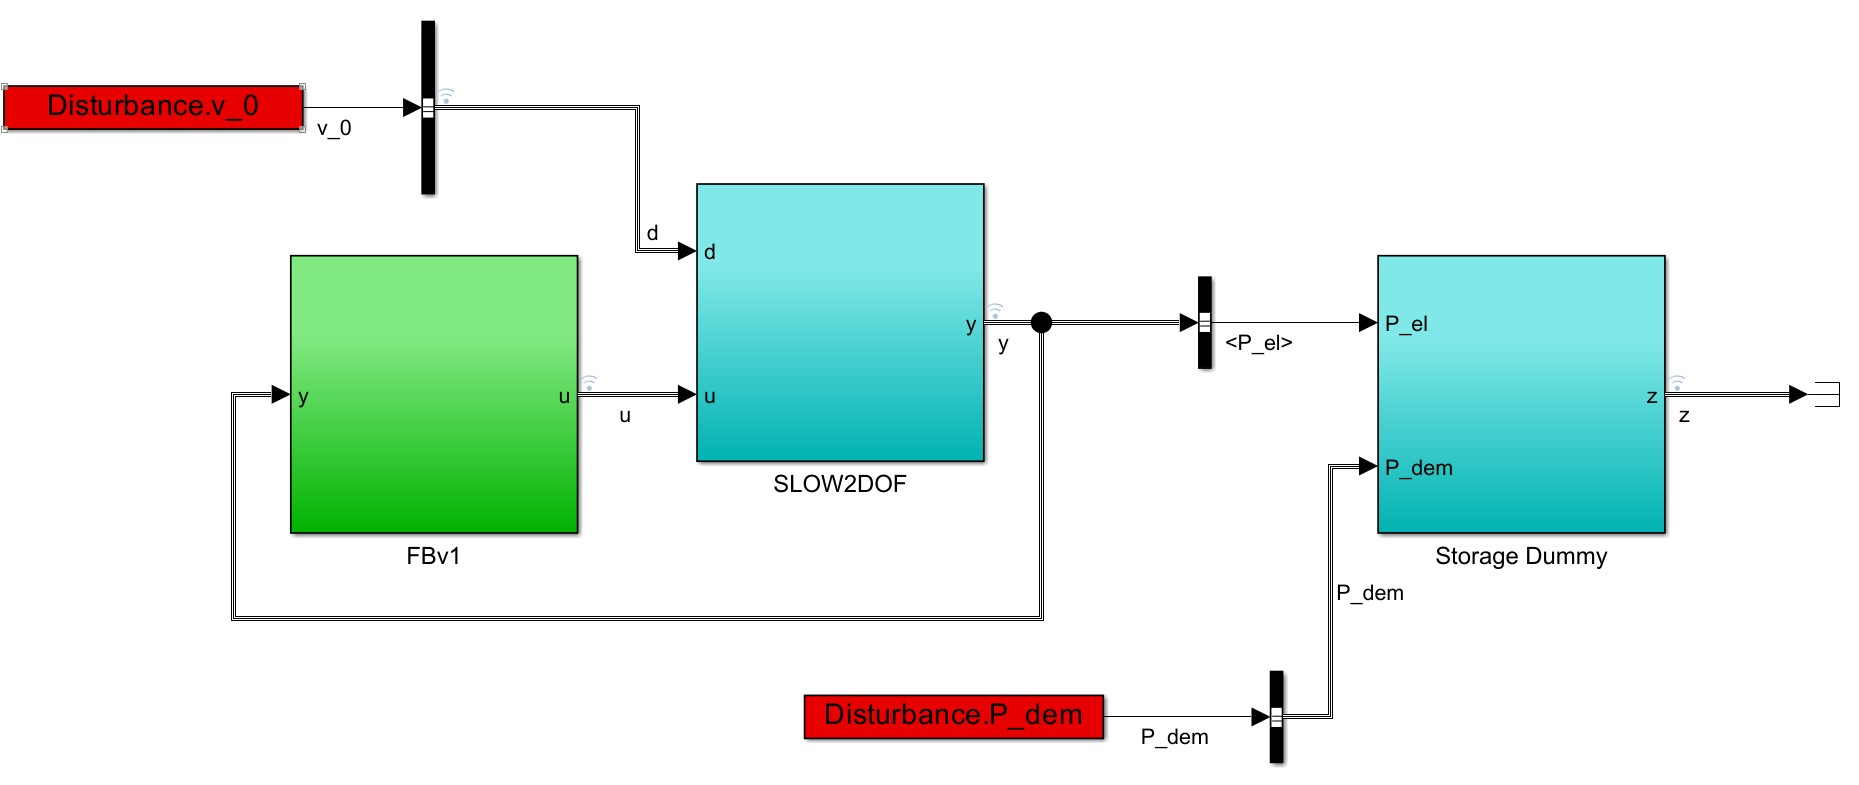
\includegraphics[width=12cm]{Figures/StorageDummy}
	\caption{SSD in Simulink model}
	\label{fig:Storage dummy}
\end{figure} 

\subsection*{Description}
The \gls{SSD} was realized by a simple \gls{BMS} in combination with a integrator block.
The \gls{BMS} is capable to simulate the storage in 3 states \textit{standby}, \textit{charge} and \textit{discharge}.

\subsection*{Scenarios}
In order to explore different possibilities in which the storage system could be applied multiple scenarios where implemented into the simulation model.
A curtailment event as described in scenario 5 is shown in figure \ref{fig:curtailment scenario}.

\begin{enumerate}
	\item \textbf{No grid power demand:}
	The storage system is in working condition.
	The storage system is not at full capacity.
	There is no power infeed into the grid.
	The storage is getting charged.
	
	\item \textbf{Rated power demand from grid:}
	The storage system is in working condition.
	There is rated power feed into the grid.
	The storage is not getting charged.
	
	\item \textbf{50 \% of rated power demand from grid:}
	The storage system is in working condition.
	The storage system is not at full capacity.
	There is a power demand from the grid of \SI{50}{\%} of rated power.
	The storage is getting charged with a reduced rate of charge.
	
	\item \textbf{Turbine operated below rated power, grid demand is exceeding production:}
	The storage system is in working condition.
	The storage is charged to \SI{50}{\%} of its maximum capacity.
	The \gls{WT} is operating below rated power and the grid demand is higher than the power production of the \gls{WT}.
	The storage system is getting discharged.
	
	\item \textbf{Curtailment scenario of 4h in 25h period:}
	The storage system is in working condition.
	The storage system is not at full capacity.
	The WT is operating at rated power.
	The power must be reduced for a certain amount of time because of a curtailment order from the grid operator.
	The storage system is getting charged.
\end{enumerate}

\begin{figure}[h]
	\centering	
	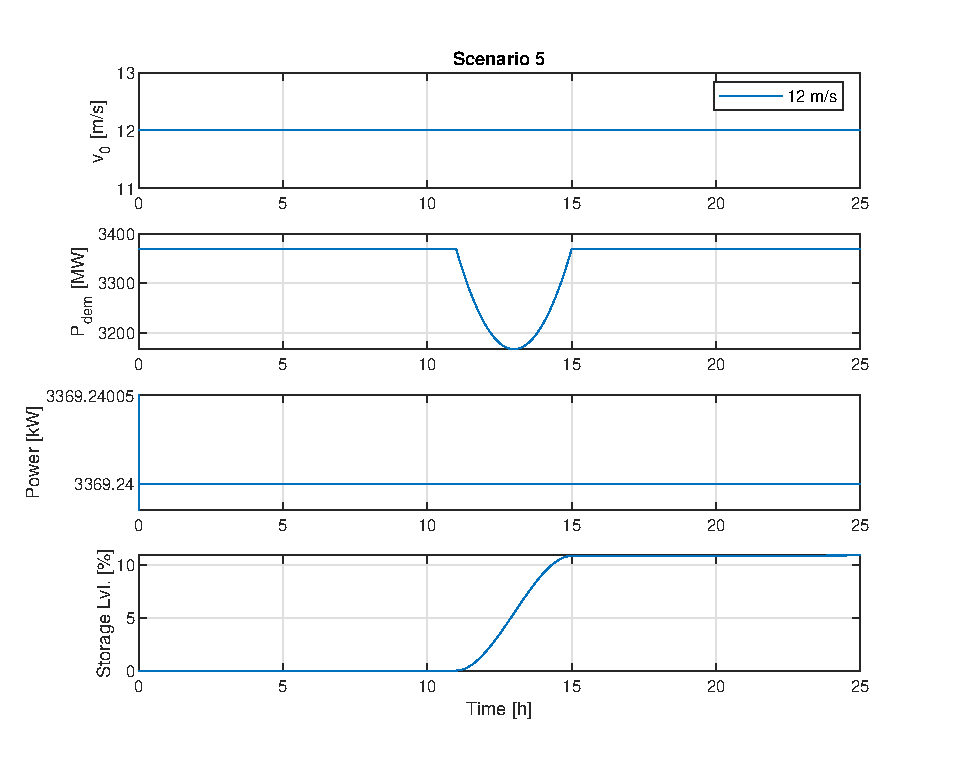
\includegraphics[width=12cm]{Figures/StorageDummyCurtailmentScenario.eps}
	\caption{Curtailment scenario for 4h duration, a storage capacity of \SI{5}{MWh} and a curtailment rate of \SI{6}{\%}.}
	\label{fig:curtailment scenario}
\end{figure} 
